\chapter{Simulationsumgebung (Omnet++)}

Um eine Simulation in einem geeigneten zeitlichen Rahmen erstellen zu können, bietet sich die Verwendung von einer Simulationsumgebung an. Diese enthält hauptsächlich ein Framework mit vielen Bibliotheken, welche für den speziellen Anwendungsfall viel Arbeit ersparen können. So bieten Simulationsumgebungen für Netzwerke beispielsweise viele Funktionen zum Anlegen von Knotenpunkten, welche wiederum verbunden werden können um miteinander zu kommunizieren.\newline
Ebenfalls oft enthalten sind eine IDE, welche unter Umständen auch spezielle Sprachen unterstützt, wie zum Beispiel die Netzwerkbeschreibungssprache NED in Omnet++. Eine weitere nützliche Funktionalität ist das generieren einer Simulation in Form einer grafischen Oberfläche, sodass Informationen nicht nur aus Dateien ausgelesen werden können, sondern für den Nutzer auch auf den ersten Blick sichtbar sind.

\section{Alternativen zu Omnet++}

Neben Omnet++ gibt es natürlich auch viele weiter Umgebungen zum Simulieren von Netzwerken. Zunächst werden hier 3 alternativen zu der in der Arbeit benutzten Umgebung Omnet++ vorgestellt: die \textbf{IKR Simulation Library (IKR SimLib)} von der Universität Stuttgart, der \textbf{Open Source Wireless Network Simulator} kurz \textbf{openWNS} von der Universität Aachen und \textbf{ns-3} vom ns-3 project.

\paragraph{Simulation Library (IKR SimLib)\cite{ikr}}

Eine freie Simulationsbibliothek unter der Lizenz GNU LGPL für Kommunikationsnetzwerke in C++ und Java von der Universität Stuttgart. Diese steht für Linux und Unix(-artige) Systeme zur Verfügung, während die Verwendung unter Windows nicht offiziell getestet wurde.\newline
Da es lediglich eine Bibliothek für Java darstellt existiert keine extra IDE und auch keinerlei GUI oder ähnliche Hilfswerkzeuge. Allerdings kann ein Projekt mit jeder normalen Java- oder C++ IDE benutzt werden, schließlich muss nur die Bibliothek importiert werden.\newline
Da schon seit den 1980ern an IKR SimLib entwickelt wird, kann die Bibliothek weitreichende Funktionalitäten zur Verfügung stellen, wie zum Beispiel Unterstützung für mobile, IP- oder P2P-Netzwerke.

\paragraph{openWNS\cite{openwns}}

OpenWNS ist ein Simulator für kabellose Kommunikation, entwickelt von der Universität Aachen. Das Projekt steht kostenlos zur Nutzung bereit und ist mit der LGPLv2 lizensiert. \newline
Es wurde speziell für Linux entwickelt, es läuft allerdings auch unter Windows. Die Entwicklung erfolgt in Python. Für grafische Unterstützung sorgt das integrierte Tool Wrowser\cite{wrowser}, welches in erster Linie dazu dient die Resultate der Simulation zu sammeln und die Messwerte zu visualisieren, aber auch beim Erstellen einer Simulation Hilfestellungen bietet, wie beispielsweise beim Einrichten der Simulationsdatenbank.\newline
Es gibt keine extra für openWNS erstellte oder angepasste IDE, allerdings wird in der Dokumentation beschrieben, wie der Texteditor Emacs\cite{emacs} den speziellen Anforderungen vom openWNS-Stil angepasst werden kann. Allerdings ist es notwendig für die Entwicklung stets einen Texteditor, den Wrowser und die Kommandozeile zu benutzen, was im Vergleich zu einer alles umfassenden IDE deutlich weniger komfortabel ist.

\paragraph{NS-3\cite{ns3}}

ns-3 ist ein freier Netzwerksimulator, der unter der GPLv2 lizensiert ist. Das Erstellen der Simulationen funktioniert mit Hilfe der Sprache Python. Dafür steht keine extra IDE zur Verfügung, was allerdings auch nicht notwenig ist, da es genügend andere Python-Umgebungen gibt.\newline
Es werden sowohl kabelgebundene als auch kabellose Verbindungen unterstützt. Allerdings besteht nicht für alle wichtigen Protokolle eine Unterstützung, wie beispielsweise WSN.\newline
Ein weiterer großer Nachteil ist, dass es keine Oberfläche während der Ausführung gibt. Die Simulation wird per Textausgabe auf der Kommandozeile ausgeführt. Die gesammelten Daten können anschließend mit Plot-Tools visualisiert werden. Für das generieren von Netzwerken steht jedoch ein grafisches Hilfsmittel zur Verfügung. Mit dem Topology Generator\cite{TopGen} können per GUI Netzwerke angelegt werden und anschließend in C++ oder Python-Code umgewandelt werden. 

\begin{table}[!ht]
  \centering
  \caption{Übersicht Simulatoren}
\begin{tabularx}{\textwidth}{lllll}
	\toprule
	& Omnet++ & IKR SimLib & OpenWNS & NS-3 \\
	\midrule
	\specialcell{free}  & \cmark & \cmark(LGPL) & \cmark (LGPLv2) & \cmark (GPLv2) \\
	\specialcell{alle gängigen\\Betriebssysteme} & \cmark & \specialcell{kein\\Windows} & \cmark & \specialcell{kein\\Windows} \\
	\specialcell{GUI bei Simulation} & \cmark & \xmark & (\cmark) & \xmark \\
	IDE & \cmark & (\xmark) & (\xmark) & (\cmark) \\
	Drahtlose Verb. & (\cmark) mit MiXiM & \cmark & \cmark & \cmark \\
	Sprache(n) & C++ mit NED & C++ oder Java & Python & Python \\
	\bottomrule
\end{tabularx}
\end{table}

\paragraph{weitere}

Es gibt natürlich außer den bisher genannten Simulationsumgebungen auch noch weitere, auf die hier aber nicht näher eingegangen werden soll. So gibt es beispielsweise GloMoSim, welches die parallele Programmiersprache Parsec benutzt. Es ist geeignet um sowohl kabellose, als auch -gebundene Netzwerke zu simulieren, jedoch wird es zum aktuellen Stand nicht mehr weiterentwickelt. \newline
Eine weitere Alternative wäre NetSim, welches von Tetcos, zusammen mit dem Indian Institute of Science entwickelt wurde. Die bestehenden Bibliotheken sind in C geschrieben und implementieren viele Protokolle wie beispielsweise WLAN, TCP oder LTE.

\section{Omnet++}

\subsection{Einleitung}

Für diese Arbeit ist Wahl allerdings auf Omnet++ gefallen. Omnet++\cite{omnet} ist eine C++-Bibliothek und ein C++-Framework, welches primär zum Simulieren von Netzwerken dient. Außerdem bietet es eine Netzwerkbeschreibungssprache namens NED (NEtwork Description) und eine auf Eclipse\cite{eclipse} basierende Entwicklungsumgebung. Für die Simulation besteht außerdem ein grafisches Interface, mit dem die Kommunikation der Knoten im Netzwerk gut verfolgt werden kann.
\newline Standardmäßig werden keine mobilen oder kabellosen Protokolle in Omnet++ unterstützt. Jedoch kann mit Hilfe des MiXiM-Frameworks die Funktionalität um eben Diese erweitert werden.
\newline Es bietet unterstützt alle gängigen Betriebssysteme wie Linux, andere Unixbasierte Systeme, Mac OS und Windows und besitzt außerdem eine kostenlose Lizenz.

\subsection{NED language}

Die Netzwerkbeschreibungssprache NED\cite{ned} bietet eine Möglichkeit auch komplexe Netzwerke relativ einfach zu beschreiben und darzustellen. Man kann schnell ein einfaches Modul mit Gates (siehe Listing \ref{lst:simpleNode}) für die Kommunikation beschreiben oder ihm Submodule für verschiedene andere Aufgaben zuweisen und dieses in ein Netzwerk integrieren und dort mehrere und auch verschiedene Instanzen von Modulen verknüpfen (siehe Listing \ref{lst:simpleNetwork}). 
\newline
Dabei helfen die verschiedenen möglichen Module. Es können die 3 Typen simple, module und network definiert werden. Wie der Name schon sagt ist network dazu da ein Netzwerk zu beschreiben und sollte alle nötigen Module als Submodule beinhalten.
\newline
Mit dem Schlüsselwort module lassen sich komplexe Objekte beschreiben. Neben den Standardvariablen wie beispielsweise Parameter, Gates oder Connections lassen sich auch Submodule definieren. Dadurch ist es möglich verschiedene in sich abgeschlossene Moduleteile in einem großen Modul zu vereinen.
\newline
Geeignet als ein solches Modulteil ist wiederum das simple-Modul. Dieses kann keine weiteren Submodule besitzen, sondern lediglich einfache Funktionalität definieren.

\begin{minipage}{\textwidth}
\begin{lstlisting}[language=ned,caption={einfaches Modul: LED},label=lst:simpleNodeLed]
simple LED
{
	parameters:
		bool ledLeuchtet;
	gates:
		input control;
}
\end{lstlisting}
\end{minipage}
\begin{minipage}{\textwidth}
\begin{lstlisting}[language=ned,caption={einfaches Modul: Knopf},label=lst:simpleNodeButton]
simple Knopf
{
	gates:
		input buttonStateChange;
		output signal;
}
\end{lstlisting}
\end{minipage}
\begin{minipage}{\textwidth}
\begin{lstlisting}[language=ned,caption={Compound Modul},label=lst:simpleNode]
module Knoten
{
	parameters:
		string name="KnotenMitLedUndKnopf";
	submodules:
		Blinker: LED {
		}
		Button: Knopf {
		}
	gates:
		input in;
		output out;
}
\end{lstlisting}
\end{minipage}
\begin{minipage}{\textwidth}
\begin{lstlisting}[language=ned,caption={einfaches Netzwerk},label=lst:simpleNetwork]
network Netzwerk
{
	submodules:
		node1: Knoten;
		node2: Knoten;
	connections:
		node1.in <-- node2.out;
		node1.out --> node2.in;
}
\end{lstlisting}
\end{minipage}
Wenn nicht anders über den Parameter @class angegeben sucht \textbf{Omnet++} nach einer Klasse, die den gleichen Namen wie das erstellte Modul besitzt. In dieser können Funktionen deklariert und implementiert werden, die das Verhalten des Moduls beeinflusst. Welche Funktionen von \textbf{Omnet++} interpretiert werden, wird im Kapitel \ref{para:Nodes and Messages} näher erklärt.
Eine Übersicht mit Kurzbeschreibung zu den wichtigsten Schlüsselwörtern in NED in der Tabelle \ref{tab:NED} zu finden.

\begin{table}[!ht]
  \centering
  \caption{NED Schlüsselbegriffe}
\begin{tabularx}{\textwidth}{lll}
	\toprule
	Kategorie & Begriffe & Funktion \\
	\midrule
	\multirow{6}{*}{Modulart} & network & ein Netzwerk, 1 pro Simulation\\
	& simple & ein einfaches, eigenständiges Modul\\
	& module & ein compound Modul, kann Submodule haben\\
	& channel & beschreibt eine Verbindung zwischen Gates\\
	& channelinterface & ein Interface für Channel\\
	& moduleinterface & ein Interface für Module\\
	\midrule
	\multirow{5}{*}{\specialcell{Sections\\von\\Modulen}} & types & um eigene Typen im Modul zu definieren\\
	& parameters & Parameter des Moduls definieren\\
	& submodules & andere Module integrieren\\
	& gates & Schnittstellen für Kommunikation definieren\\
	& connections & Gates miteinander verbinden\\
	\midrule
	\multirow{3}{*}{Typen} & \multicolumn{2}{l}{int, string, double, bool}\\
	& xmldoc & speichert den Pfad eines XML-Files\\
	& xml	 & speichert XML\\
	\midrule
	\multirow{5}{*}{Verbindungen} & allowunconnected & \specialcell{erlaubt Kommunikation zwischen Gates \\ohne definierte Verbindung}\\
	& input & definiert ein Gate als eingehend\\
	& output & definiert ein Gate als ausgehend\\
	& inout & legt je ein in- und output Gate an\\
	\midrule
	\multirow{7}{*}{weitere} & @display & Eigenschaften zur Darstellung bei Sim.\\
	& @class & spezielle C++-Klasse zum Modul definieren \\
	&package & definiert den Namensraum\\	
	& import & andere Pakete und Module einbinden\\
	&\multicolumn{2}{l}{volatile, const, extends,import,like}\\
	&\multicolumn{2}{l}{this,false,true,default, if,and,or,else,for}\\
	&\multicolumn{2}{l}{index,sizeof,typename}\\
	\bottomrule
\end{tabularx}
\label{tab:NED}
\end{table}

\subsection{Einige Techniken, Funktionen und wichtige Module}

Im folgenden Abschnitt wird ein Ausschnitt darüber gegeben, was Omnet++ an Funktionalitäten bereitstellt. Grundlegend wird für eine einfache Simulation ein Netzwerk benötigt, welches in der Netzwerkbeschreibungssprache NED beschrieben wird. Dieses Netzwerk kann dann Nodes definieren, welche selbst Module sind, welche wiederum auch in NED beschrieben werden. Wenn diese Module ausgehende und/oder eingehende Gates besitzen, können diese im Netzwerk wiederum miteinander verbunden werden.\newline
Dieser einfache Grundaufbau genügt im Prinzip schon, damit eine valide Simulation ablaufen kann. Um dazu noch etwas Funktionalität in die Module zu bringen ist es möglich für jedes Modul eine Klasse in C++ zu definieren. Man kann zum einen eigene Klassen definieren oder die in der Simulationsbibliothek vorhandenen Klassen nutzen.\newline
Zusätzlich zur Standardbibliothek gibt es noch 3 relevante Frameworks, die weitere Funktionen zur Verfügung stellen: MiXiM, INET und Castalia.

\subsubsection{Nodes and Messages}\label{para:Nodes and Messages}

Für die Steuerung innerhalb einer Simulation sind Nachrichten das wichtigste Werkzeug in \textbf{Omnet++}. So kann man eine Nachricht zu einer festgelegten Simulationszeit verschicken, um diese als Events einzusetzen. Dabei können Knoten auch Nachrichten an sich selbst versenden.

Um einem selbst definierten Modul die Möglichkeit zu geben Nachrichten zu verstehen und zu benutzen werden einige Funktionen bereit gestellt, die man selbst definieren muss.

Diese sind für die Funktionalität eines \textbf{cSimpleModule} entscheidend und sollten nach dem Erstellen eines neuen Moduls implementiert werden:

\begin{itemize}
\item void initialize()
\item void handleMessage(cMessage *msg)
\item void activity()
\item void finish()
\end{itemize}

\paragraph{initialize()}

Die Funktion \textbf{initialize()} wird nach dem Erstellen eines Modules aufgerufen. Es kann ähnlich wie ein Konstruktor verwendet werden. Entscheidend ist, dass die Methode erst aufgerufen wird, nachdem auch der \textbf{NED}-Teil des Moduls eingelesen wurde. Das bedeuted, dass erst an dieser Stelle auf Parameter des Moduls zugegriffen werden kann und das ist im Konstruktor noch nicht möglich. Auch Nachrichten kann das Modul erst ab diesem Zeitpunkt verschicken. 

\paragraph{handleMessage(cMessage *msg)}

Diese Methode kann eingehende Nachrichten auswerten. Sollten bei einem Modul Nachrichten ankommen, ohne dass diese Funktion definiert wurde, wird ein Fehler auftreten. Wie Nachrichten genauer aufgebaut sind ist im Abschnitt \textbf{cMessage} beschrieben.
Nachrichten können zeitgesteuert Events auslösen. Die Methode \textbf{handleMessage()} ist somit das Herzstück der meisten Module, da hier das komplette Verhalten geregelt wird. \newline
Es können im Regelfall natürlich viele verschiedene Arten von Nachrichten in einem Modul eintreffen, die auch unterschiedlich behandelt werden müssen. Zur Fallunterscheidung stehen wiederum viele Funktion im Nachrichtenmodul zur Verfügung, die beispielsweise Informationen über den Sender liefer, ob die Nachricht eine Selfmessage war, also vom Modul an sich selbst gesendet wurde oder einfache Informationen wie der Name der Nachricht.

\paragraph{activity()}

Diese Methode ist eine eher unwichtige Funktion. Wenn \textbf{handleMessage()} korrekt verwendet wird, sollte man auf die Benutzung von \textbf{activity()} am besten komplett verzichten. Es verhält sich oberflächlich betrachtet wie \textbf{handleMessage()}, allerdings wird diese Methode nicht einfach aufgerufen, sollte eine Nachricht ankommen, sondern läuft in einer Endllosschleife und wartet permanet aktiv auf Nachrichten. Daher ist sie wesentlich Speicherintensiver als das Gegenstück \textbf{handleMessage()}.

\paragraph{finish()}

Diese Methode wird aufgerufen nachdem die Simulation beendet wurde und noch bevor das Modul gelöscht wurde. Sie sollte nicht zum Löschen anderer Module verwendet werden, da nach dem Aufruf von finish() die Simulation erneut gestartet werden kann, ohne das das Netzwerk komplett neu initialisiert wird. Wenn allerdings wichtige Module an dieser Stelle gelöscht wurden ist ein Neustart nicht mehr möglich.\newline
Die Methode ist stattdessen dafür da die eben abgelaufene Simulation auszuwerten. Es können an dieser Stelle alle relevanten Informationen gespeichert werden, damit diese hinterher statistisch ausgewertet werden können.

\subsubsection{cMessage}

Für die Nachrichten selbst existiert ein fertig implementiertes Modul namens \textbf{cMessage}. Dieses erfüllt schon die wichtigsten Anforderungen, die man an ein Nachrichtenmodul stellt. So können Nachrichten nicht nur \textbf{strings} übertragen, sondern alle Klassen, die von \textbf{cNamedObject} erben. Man kann also auch komplexe, selbst definierte Objekte mithilfe von cMessage übertragen.
Es empfiehlt sich dennoch eine eigene Kindklasse von cMessage zu definieren, da man in diesem eigene Parameter definieren kann, die verschiedene Werte beschreiben. So kann man zum Beispiel genauere Informationen für Quelle und Senke in der Nachricht speichern oder verschiedene Werte für Statistiken. Sollte man eine veränderte Kindklasse von cMessage definieren, so wird zusätzlich eine Klasse dazu generiert, die viele Funktionen bereitstellt, die zum Beispiel das kopieren einer Nachricht ermöglichen - auch inklusive der extra hinzugefügten Parameter.

\begin{table}[!ht]
  \centering
  \caption{Übersicht über einige Funktionen von cMessage}
\begin{tabularx}{\textwidth}{rll}
	\toprule
	typ & Funktion & Kurzbeschreibung\\
	\midrule	
	virtual cArray \& & getParList () & Parameterliste einer Nachricht\\
	bool 	& isSelfMessage () const & ist Nachricht an sich selbst\\
	cModule * 	& getSenderModule () const & \multirow{4}{*}{\specialcell{Informationen über Sender\\äquivalent für Arrival vorhanden}} \\
	cGate * 	& getSenderGate () const  & \\
	int &	getSenderModuleId () const & \\
	int &	getSenderGateId () const & \\
	simtime\_t\_cref 	& getCreationTime () const & Zeitpunkt: Nachricht erstellt\\
	simtime\_t\_cref 	& getSendingTime () const & Zeitpunkt: Nachricht gesendet\\
	simtime\_t\_cref 	& getArrivalTime () const  & Zeitpunkt: Nachricht angekommen\\
	bool &	arrivedOn (int gateId) const & Id des Inputgate\\
	\bottomrule
\end{tabularx}
\end{table}

\subsubsection{Event}

Die Zeit einer Simulation verläuft linear. Anhand dieser kann die Ausführung von Events für einen bestimmten Zeitpunkt geplant werden. Dies ist möglich durch das Versenden von cMessage in Kombination mit einer Scheduletime und wenn nötig als Selfmessage.\\
Wenn ein Modul einen Zeitraum der Ausführung abgeschlossen hat, soll es unter Umständen eingefroren werden und erst zu einem späteren Zeitpunkt reaktiviert werden. Damit es in dieser Zeit nicht aktiv warten muss und somit unnötig Prozessorlast oder im Fall von mobilen Geräten auch noch zusätzlich Energie verbraucht, kann ein Modul jegliche Aktionen unterlassen, bis eine Nachricht, wie ein Event, die weitere Ausführung wieder anstößt (siehe Abbildung \ref{fig:messageEvent}). 

\begin{figure}[htbp]
\centering
\caption{Beispiel cMessage als Event}
\label{fig:messageEvent}
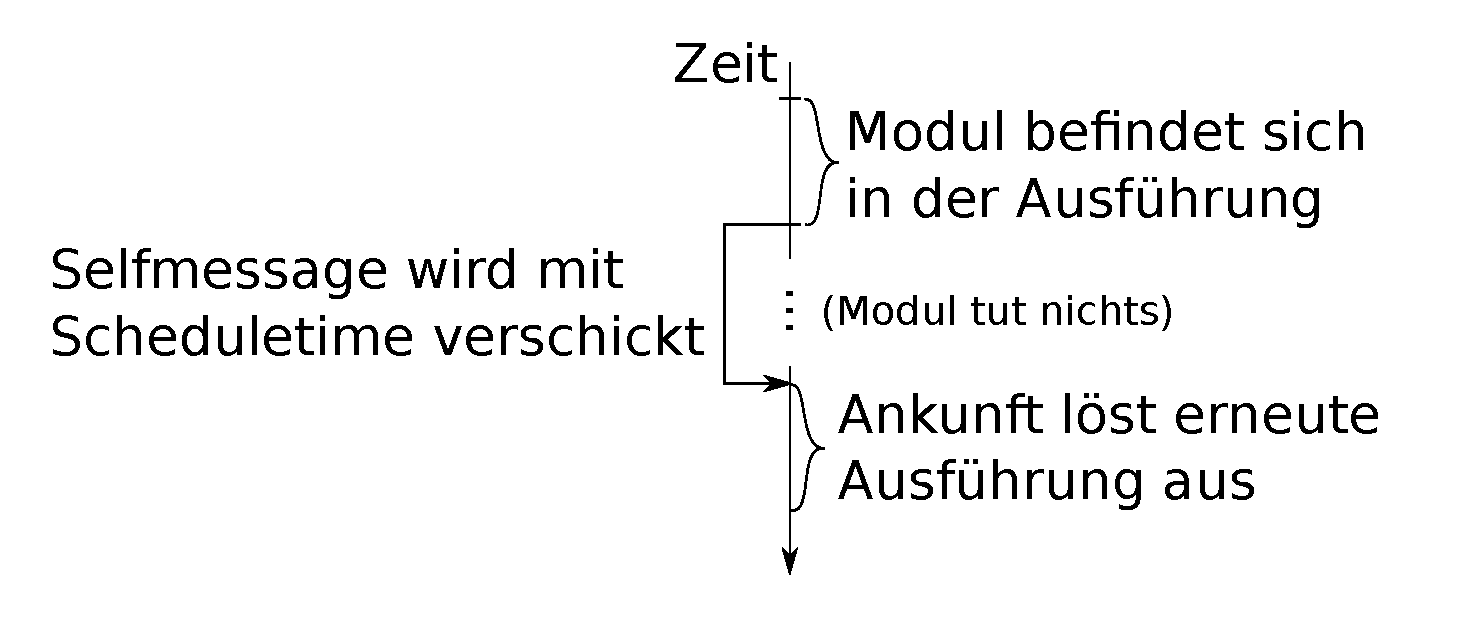
\includegraphics[width=\textwidth]{messageEvent}
\end{figure}

\subsubsection{XML Support}

NED-Parameter eines Moduls können vom Typ xml sein. Die dazu gehörende Klasse cXMLElement bietet ihrerseits umfangreiche Unterstützung dafür an. Diese orientiert sich dabei an einem DOM-Parser, ist allerdings aus Performanzgründen nur ähnlich aufgebaut. Dabei stellt die Klasse die für X-Path typischen Funktionen für XML-Zugriffe bereit wie zum Beispiel \textbf{getParentNode()} oder \textbf{getChildren()}.

\begin{minipage}{\textwidth}
\begin{lstlisting}[language=C++,caption={Beispiel einlesen von XML},label=lst:xml]
cXMLElement *rootE = par("xmlFile").xmlValue();
cXMLElementList nListRows = rootE->getChildren();
int amountRows = nListRows.size();
int* data = new int[amountRows];
for (int i = 0; i < amountRows; i++){
    //nListRowArray ist eine Zeile aus dem XML file 
    //bzw. alle Elemente 1. Ebene unter der Wurzel
    cXMLElement* nListRowArray = nListRows[i];
    //kann ab hier beliebig tief fortgesetzt werden
}
\end{lstlisting}
\end{minipage}

\section{MiXiM-Framework als Omnet++-Erweiterung}

\subsection{Einleitung}

MiXiM\cite{mixim} ist ein Framework welches die Funkionalität von Omnet++ in erster Linie um mobile und kabellose Knoten erweitert. Es implementiert einige Protokolle und stellt verschiedene Knoten bereit.\\
Außerdem fügt es zusätzlich auch nützliche Hilfsfunktionen zu Omnet++ hinzu, wie beispielsweise die FindModule-Klasse.

\subsection{Einige wichtige Module}

\subsubsection{FindModule}

Diese Klasse kann eine Instanz eines Objekts anhand eines Modulnamens finden. Es verhält sich daher wie eine Art Servicemanager. Mann kann mit Hilfe Dieser Submodule, globale Module, Hostmodule und Netzwerke finden. Dazu übergibt man einfach an ein Template wie in Beispiel \ref{lst:findmodule} den gewünschten Modulnamen und kann dann eine der Methoden, wie zum Beispiel findSubModule() aufrufen.

\begin{lstlisting}[language=C++, caption={Beispiel FindModule}, label=lst:findmodule]
//template der FindModule Klasse
template<typename T = cModule * const >
//Beispielverwendung
FindModule<BasePhyLayer*>::findSubModule(this)
\end{lstlisting}

\subsubsection{Coord}

Coord ist eine einfache Klasse zur Repräsentation von Koordinaten im 3-dimensionalen Raum. Es ist eine elementare Klasse für das MiXiM-Framework, da dieses Mobilität implementiert. Coord beinhaltet zusätzlich zu den 3-D-Koordinaten auch beispielsweise untere und obere Grenzen, Operatoren zum rechnen und vergleichen und weitere Methoden wie zum Beispiel eine Distanzberechnung zwischen Koordinaten.

\subsubsection{Mobility}

Wie im vorherigen Abschnitt schon erwähnt ist die Mobilität eine der wichtigsten Funktionen, die das MiXiM-Framework bereitstellt. Es werden 4 verschiedene Arten von Bewegungen zur Verfügung gestellt, wobei eine davon, die LineSegmentMobilityBase, selbst wiederum viele verschiedene Varianten zur Verfügung stellt: 
\begin{itemize}
\item CircleMobility
\item LinearMobility
\item RectangleMobility
\item LineSegmentMobilityBase
\end{itemize}
Während die ersten 3 Arten sich von selbst erklären, ist dass bei der LineSegmentMobilityBase nicht der Fall. Es ist eine weitere Basisklasse für Bewegungsarten welche aus einer Sequenz verschiedener linearer Bewegungen bestehen. Ein Beispiel ist die sogenannte TurtleMobility. Bei dieser kann ein Skript als XML-File hinterlegt werden, welches die Sequenz beschreibt.

\subsubsection{Wireless}

BaseArp
src/modules/node/Host80211.ned

\paragraph{Host80211}

IEEE 802.11
Norm für Funknetzwerke

\todo{Ergänzen}









